\section{Background}
\subsection{Neural Network}
We conceptualize neural networks as directed acyclic graphs 
comprising three types of layers: the input layer, intermediate hidden layers, 
and the output layer. Our goal is to focus on the abstracting feed forward networks, 
where neuron values are computed based on preceding layer neuron values. 
Neurons in our network are denoted as $n_{(i,j)}$, where `$i$' signifies the 
neuron number in layer `$j$'. The weight matrix between layers `${j-1}$' and `$j$' 
is denoted as `$W_{{j-1}, j}$', and the bias matrix for layer `$i$' is denoted as 
`$B_{i}$'. The value of the `$i^{th}$' neuron in layer `$j$' is represented by 
`$v_{(i,j)}$', and `$V_{j}$' encompasses all such `$v_{(i,j)}$' values for layer 
`$j$'.

The computation of `$V_{j}$' involves applying an ``activation function ($\phi$)" 
to the ``weighted sum":

\[V_{j} = \phi(W_{{j-1}, j} \cdot V_{j-1} + B_{j}).\] 

We confine our activation function to the Rectified Linear Unit (ReLU), 
which can be expressed as $V_{j} = \max(W_{j-1, j} \cdot V_{j-1} + B_{j}, 0)$.


\begin{figure}[H]
    \centering
    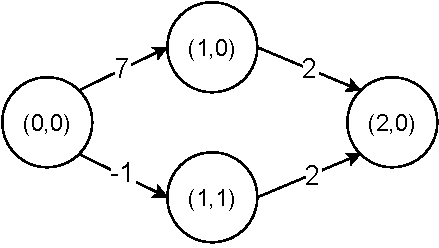
\includegraphics[width=0.3\textwidth, height = 0.15\textwidth]{diagrams/Basic_Neural_Network.pdf}
    \caption{A Simple Neural Network}
    \label{Figure: Simple Neurla}

\end{figure} 

Figure \ref{Figure: Simple Neurla} depicts a feed forward neural network 
comprising four neurons: $n_{(0, 0)}$, $n_{(1, 0)}$, $n_{(1, 1)}$, and $n_{(2, 0)}$. 
The weight matrix between layer 0 and layer 1, denoted by $W_{0,1}$, 
is $[7, -1]^T$, and the bias matrix for layer 1, denoted by $B_{1}$, 
is $[0, 0]^T$. If we assign a value of 1 to the neuron $n_{(0, 0)}$ 
(i.e., $v_{(0, 0)}=1$), then the value of the neuron $n_{(1,0)}$ is $v_{(1,0)}=7$, 
as determined by $V_{1} = \phi([7, -1]^{T} \cdot [1] + [0, 0]^{T}) = [7, 0]^{T}$.


\subsection{Neural Network Verification }
In the context of neural network verification, we typically engage with a
 neural network, posing a ``$\textit{satisfiablility}$'' query to validate or 
 refute a property. The query \(\mathcal{P}\) is structured as a triple,
  \(\mathcal{P} = \langle \mathcal{N}, \kappa, \lambda \rangle\). Here,
   \(\mathcal{N}\) denotes the neural network as previously mentioned, 
   while \(\kappa\) and \(\lambda\) represent properties on the input and 
   output neurons, respectively. 

$\kappa$ is defined as a conjunction of linear constraints applied to the 
input neurons. Correspondingly, $\lambda$ is also expressed as a conjunction 
of linear constraints targeting the output neurons. Our objective is to verify
boolean properties formulated as $\forall x \in X,\textit{ } y < c$. However, 
for the purpose of assessing the validity of these properties, we transform 
our $\lambda(y)$—the conjunction of constraints on our output variables—into
the negation of $y < c$, represented as $y \geq c$, where $y$ denotes the output 
of the neural network. To achieve this transformation, we introduce additional
neurons into the network, resulting in a modified network structure with a singular
output neuron. This transformation of the Neural Network $\mathcal{N}$ proves 
advantageous for subsequent Inc/Dec classification, which is described in the
subsequent section 2.3.1.

Our query is constructed as a boolean formula 
\(\mathcal{P}(x) \equiv \kappa(x) \land \lambda(\mathcal{N}(x))\). 
Since we are looking for validity we use the negation of the output 
property and seek an `UNSAT'. The solver is presented with the formula 
\(\exists x \in X, \mathcal{P}(x)\), where \(X\) is the domain of the input. 
If our solver responds with `SAT' to this query, it indicates that we have 
identified a counterexample, and our property does not hold. Conversely, an
 `UNSAT' result signifies the validity of our original property.


\subsection{Counter-example guided abstraction and refinement}
To aid and expedite the verification queries, we employ a strategy to simplify 
our neural network by reducing the number of neurons. Our approach involves
 constructing an over-approximate network, denoted as $\mathcal{N''}$, where 
 the output value, $\mathcal{N''}(x)$, consistently exceeds the value computed 
 by the original network, $\mathcal{N}(x)$, i.e ($\forall x \in X, \hspace{1mm} 
 \mathcal{N''}(x) \geq \mathcal{N}(x)$), where $X$ is our input domain. This
  simplification is undertaken because our property which is expressed as
   $\forall x \in X, \hspace{1mm} \mathcal{N}(x) < c$ can then be proven by 
   determining the unsatisfiability of $\exists x \in X, \hspace{1mm}\mathcal{N''}(x)
 \geq c$. If the answer to this question is `Yes,' then it implies that
  $\forall x \in X, \hspace{1mm} \mathcal{N}(x) < c$ holds, as evidenced by 
  ($\forall x \in X, \hspace{1mm} \mathcal{N''}(x) \geq \mathcal{N}(x)$).



\subsubsection{Increment Decrement Splitting}
To aid in the process of constructing such an over-approximate network 
we begin with the creation of an equivalent network, denoted as $\mathcal{N}'$,
 ensuring that $\mathcal{N'}(x)$ equals $\mathcal{N}(x)$ for all $x$.
To build this equivalent network, we perform an `Increment/Decrement'
splitting of neurons in our original network $\mathcal{N}$. Upon reflection, 
it became apparent to us that a two-class classification was more fitting for 
our needs, deviating from the initially recommended four-class classification 
outlined in the original work by \cite{b2}. Neurons are categorized as 
`Increment (Inc)' if increasing their values increases the output neuron's value,
 and as `Decrement (Dec)' if decreasing their values achieves the same result.

\begin{algorithm}[H]
    \caption{split\_Inc\_Dec}
    \begin{algorithmic}[1]
        \State Initialize M, the set of nodes that are marked, to \{out\_node\} and mark out\_node as \textbf{Inc}.
        \State Let $R$ be the set of nodes with successors in $M$.
        \State Define $\text{sign(u,v)}$ as the sign of the weight from the node $u$ to $v$.
        \State Define $\text{Class(v)}$ as $1$ when $v$ is marked as $\textbf{Inc}$, and $-1$ otherwise.
        \While {\text{node} $\notin M$ and node $\notin$ input\_nodes}
        \State Pick a node $u$ such that $u \in R-M$
        \State Suppose $u$ feeds into $x_1,x_2,x_3,..$ and $y_1,y_2,y_3..$ where $\text{sign($u,x_i$)} = \text{Class($x_i$)}$ for all $x_i$, $\text{sign($u,y_i$)} \neq \text{Class($y_i$)}$ for all $y_i$.
        \State Split $u$ to $u_1$ and $u_2$, where $u_1$ feeds into all the $x_i$ and $u_2$ feeds into all the $y_i$.
        \State Mark $u_1$ as \textbf{Inc} and $u_2$ as \textbf{Dec}
        \State Insert $u_1$ and $u_2$ into $M$ and their predecessors into $R$
        \EndWhile
        \end{algorithmic}
\end{algorithm}


\subsubsection{Abstraction}

\begin{figure}[H]
    \centering
    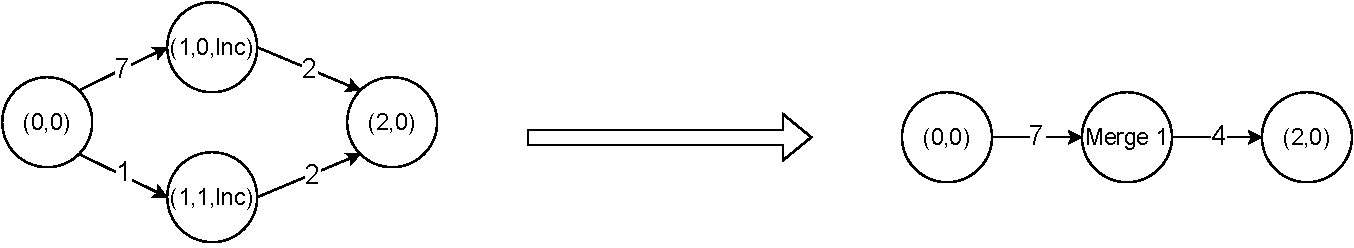
\includegraphics[width=0.5\textwidth]{diagrams/Abstraction_part1.pdf}
    \caption{Merging of Increment Neurons}
    \label{Figure: Merge1}
    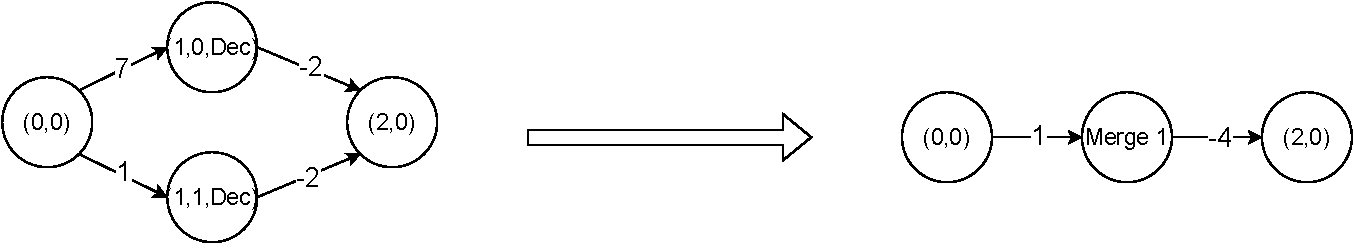
\includegraphics[width=0.5\textwidth]{diagrams/Abstraction_part2.pdf}
    \caption{Merging of Decrement Neurons}
    \label{Figure: Merge2}

\end{figure} 
The increment/decrement splitting of the neural network $\mathcal{N}$ to 
the new network $\mathcal{N'}$ changes the structure of the neural network but
 does not change the value of the output neuron. If we want to construct
  a neural network $\mathcal{N}''$ which over-approximates the value of 
  the original network $\mathcal{N}$ i.e $\forall x \in X, \hspace{1mm} 
  \mathcal{N''}(x) \geq \mathcal{N}(x)$, then we perform the following steps:
\begin{enumerate}
    \item When merging two $\textit{Increment Neurons}$, discard one of those neurons and replace the incoming weight by maximum of all the incoming weights and the outgoing weight by summation of all the outgoing weights. 
    \item When merging two $\textit{Decrement Neurons}$, discard one of those neurons and replace the incoming weight by minimum of all the incoming weights and the outgoing weight by summation of all the outgoing weights. 
\end{enumerate}


\subsection{Refinement }
After merging the neurons, we introduce an over-approximation into 
the new network $\mathcal{N''}$. And since $\mathcal{N''}(x) \geq \mathcal{N}(x)$,
 there might exist a $x$, for which, $\exists x \in X, \hspace{1mm} \mathcal{N''}(x)
\geq c$ but $\nexists x \in X, \hspace{1mm} \mathcal{N}(x) \geq c$. 
Therefore, if a counter-example `$\beta$' returned is not a valid counter-example,
which means, $\mathcal{N''}(\beta) \geq c > \mathcal{N}(\beta)$, then, we must 
reverse some of the merges performed previously to get a new network which mitigates
the extent of the over-approximation for us to get a valid counter-example or to 
prove that the original property is valid.

In \cite{b2}, the authors employed a Counterexample-Guided Abstraction 
Refinement (CEGAR) approach to eliminate the spurious counter-examples. 
They utilized a counter-example ($\beta$) to identify a neuron $n_{(i, j)}$ 
that had been merged into the node `$r$' for refinement. The authors then 
computed the value $\omega$ which was equal to 
$|v_i^j(\beta) - r(\beta)| \cdot |w_{n_{(i-1, k)},n_{(i,j)}}-w_{n_{i-1,k},r}|$, 
where $v_{(i, j)}(\beta)$ denotes the value of $n_{(i, j)}$ at the 
counter-example $\beta$, $r(\beta)$ denotes the value of the 
representative neuron $r$ at the counter-example $\beta$, $w_{n_{(i-1,k)},n_{(i,j)}}$ 
denotes the weight between a neuron $n_{i-1,k}$ and a neuron $n_{i,j}$. 
If this value $\omega$ was over a recommended amount $\epsilon$, they proceeded to 
separate $n_{(i, j)}$ from $r$ to potentially eliminate the spurious counter-example 
$\beta$.

\dmcmt{ 
    An example of Elboher's Refinement where we get a lot of singletons
}


 In the next section, we present a new method for merging neurons in 
 order to reduce the number of refinement steps, thereby expediting the 
 verification process.
